%definición del artículo
\documentclass[a4paper,12pt,openany,oneside]{book}
\usepackage[left=5cm,right=2cm,top=4cm,bottom=4cm,paperwidth=216mm,paperheight=330mm,pdftex]{geometry}
%paquete usado para silabación en español
\usepackage[spanish]{babel}
%codificación del documento
\usepackage[utf8]{inputenc}
%espaciado
\linespread{1.5}
%identación de párrafo
\setlength{\parindent}{20pt}
%espaciado de párrafo
\setlength{\parskip}{4ex plus 0.5ex minus 0.2ex}
%para validar sólo sintaxis sin compilar
%\usepackage{syntonly}
%\syntaxonly
%para usar imágenes
\usepackage{graphicx}
%para usar fragmentos de codigo fuente
\usepackage{listings}
\usepackage{float}
%para usar signos de check y wrong
\usepackage{bbding}
%para usar colores en textos y simbolos
\usepackage{color}
\usepackage{multirow} %multi columna
\floatstyle{boxed}
\newfloat{codigo}{thp}{lop}
\floatname{codigo}{Caja de Código}

%comienzo del documento
\begin{document}
%\thispagestyle{empty}

\begin{center}
\textbf{UNIVERSIDAD TECNOLÓGICA METROPOLITANA\\
FACULTAD DE INGENIERÍA\\
ESCUELA DE INFORMÁTICA}\\
\vspace{3cm}
MÓDULOS INTEGRADOR Y MANTENEDOR DE DATOS EN SISTEMA S.E.P.A.
\end{center}
\begin{flushright}
TRABAJO DE TÍTULO PARA OPTAR AL TÍTULO DE\\
INGENIERO CIVIL EN COMPUTACIÓN MENCIÓN INFORMÁTICA\\
\vspace{3cm}
PROFESOR: Sebastián Salazar Molina\\
\vspace{1.5cm}
ALUMNO: Miguel Ángel Aníbal Davor Fuenzalida Pino
\end{flushright}
\vspace{4cm}
\begin{center}
SANTIAGO - 2015
\end{center}
\newpage
\thispagestyle{empty}
\begin{flushright}
\vspace{20mm}
Nota: \line(1, 0){140} \\
\vspace{30 mm}
\line(1, 0){180}\\	
Firma y Timbre\\
Autoridad Responsable
\end{flushright}
\chapter*{Resumen}
\thispagestyle{empty}
En las organizaciones es necesario el uso de información para tomar decisiones correctas. Tener un buen software, entrega valor agregado a la dirección de actividades en todo tipo de estructuras con jerarquía.

La UTEM dispone del sistema S.E.P.A. (Sistema Estadístico de Profesores y Alumnos), que consiste en un proyecto Web realizado con la herramienta PHP que toma datos de alumnos, profesores y encargados provenientes de DirDoc, para posteriormente hacer cálculos predefinidos para obtener indicadores que representen la realidad universitaria.

Sin embargo S.E.P.A. presenta insuficiencias, por ejemplo: no dispone de un servicio web (una forma de acceso más segura y controlada) que se comunique con DirDoc o no presenta formas alternativas de acceso, no tiene multiroles y presenta datos incompletos.

% ejemplos, no tiene servicio web dirdoc, inconsistencia de datos, carece de formas alternativas de accesos, carece multiples roles (más de 2).

El presente trabajo de Título ofrece una mejora al sistema S.E.P.A., con integración de herramientas que permiten mejoras por la Universidad (serán explicadas a fondo en este documento). Las herramientas usadas en este proyecto son: 

\begin{itemize}
	\item El sistema gestor de bases de datos PostgresSQL.
	\item Herramienta de construcción de proyectos MAVEN para el lenguaje de programación Java.
	\item Uso de servicios web con CXF.
\end{itemize}

El resultado final de este proyecto es la obtención por parte de la Universidad un webservice que comunique S.E.P.A. con DirDoc de manera mas expedita y segura, mediante varios tipos de consultas, un módulo de mantenedor que permitirá monitorizar y editar las distintas tablas, con sus registros correspondientes, pensado desde un principio para hacer búsquedas y reparar data que este incompleta.

\tableofcontents
\listoffigures
\chapter*{Introducción}
\thispagestyle{empty}
La Universidad Tecnológica Metropolitana utiliza para la administración de toda la información referente a estudiantes, profesores y personal de administración un sistema denominado DirDoc basado en la tecnológica PHP. S.E.P.A., software desarrollado por Sebastián Salazar Molina para en ese entonces su trabajo de título, es un proyecto que constituyó una forma de potenciar las capacidades operativas de la Universidad, generando indicadores de calidad y entregando una ventaja comparativa frente a otras Universidades.

El objetivo de este trabajo de título esta en la actualización del proyecto S.E.P.A. mediante el lenguaje Java que utiliza herramientas estructuradas, extensibles y que tienen como resultado la materialización de sistemas informáticos de más fácil mantención debido al uso de Patrones de Diseño (explicados en este informe):

\begin{itemize}
	\item Modelo Vista Controlador: Es un modelo de desarrollo informático que permite separar el modelo de datos, el negocio y sus flujos, de la vista para el usuario final \cite{data12}.
	\item Java EE: Java enterprise edition, es una plataforma para programadores en Java que contiene herramientas enfocadas en el desarrollo de aplicaciones para empresas \cite{data14}.
	\item JPA: Java Persistente API, una herarmienta que permite la homologacion de la base de datos que un sistema trabaje, frente a un modelo de objetos simple creado en lenguaje Java \cite{data13}.
	\item Spring: Herramienta que permite la integración de distintos modulos en aplicaciones Java EE, entre otras utilidades, permite la separación de los componentes de desarrollo bajo el esquema MVC  \cite{data15}.
	\item JSF: Herramienta que permite desarrollar interfaces con una potente comunicación con aplicaciones Java EE bajo el modelo MVC \cite{data16}.
	\item PrimeFaces: Kit de desarrollo para aplicaciones en JSF que permite usar componentes mas avanzados y específicos que JSF \cite{data17}.
\end{itemize}

Además, el proyecto se hará bajo la metodología PSP (Personal Software Process) que nos proporciona un modelo de trabajo basado en la caracterización de los tiempos y costes de operación de un ingeniero informático, adicionando documentación extra (explicada en este informe), correspondiente a eventos que caracterizaron las directrices de cómo se lleva adelante esta tarea, todo lo cual, conduce a una evaluación de la calidad del proyecto como programa.

Existen 3 tipos de beneficios que la Universidad puede obtener al hacerse con la versión mejorada del sistema S.E.P.A.:

\begin{enumerate}
\item Mediante la entrega al mercado laborar, de un perfil de profesional característico de la U.T.E.M., visualizado en la competencia y desempeño de sus profesionales, la Universidad se muestra al mercado como un ente preocupado de medir su calidad con herramientas tecnológicas que justifican un buen desempeño mediante indicadores cuantificables y verificables por 
organismos reguladores.

\item Beneficio de los usuarios que tendrán a su disposición una completa herramienta que los apoyará en la elección de su carga académica, como asimismo la visualización de su desempeño.

\item Beneficio a futuro, dado el alto estándar de las herramientas utilizadas, la integración, en términos de programación, resultará más sencilla, ya que este proyecto está realizado bajo tecnologías más estandarizadas como lo son los proyectos desarrollados en Java, Maven y Spring.
\end{enumerate}

La justificación principal de por que en S.E.P.A. se realizarán estas mejoras, radica en la necesidad de contar con indicadores claros y precisos, que son los que hacen que las decisiones sean justificadas, Por ejemplo, una vez implementadas las mejoras, en S.E.P.A. se prodrá fácilmente programar contadores de la totalidad de las tablas, incluidas conexiones entre tablas, mientras que la version actual de S.E.P.A. tiene contadores simples y poco específicos, tales como el promedio de notas por ramo y por alumnos programados de manera tal que no se pueden hacer búsquedas especificas sobre todos los parámetros de una tabla en especifico.

Otra justificación de estos cambios, es la capacidad de reparar data que este mal escrita o que simplemente no exista, permitiendo que los datos puedan ser mejorados constantemente y de manera expedita. Característica que S.E.P.A. actual no posee, ya que para solicitar un cambio se necesita básicamente pedir la data desde la propia fuente de datos, proceso que es manual y toma días y muchas personas.

Finalmente es importante destacar que las transacciones de los servicios web que se agregaran como parte de este proyecto constituyen otra mejora, haciendo el sistema mas seguro y rápido.

\chapter{Antecedentes}
\thispagestyle{empty}
\section{Contexto General}
La Universidad Tecnológica Metropolitana (UTEM) es un organismo de enseñanza superior que se encuentra dentro del Consejo de Rectores de las Universidades Chilenas. Dentro de su sistema administrativo de notas se ocupa el sistema DirDoc, el cual entrega información de notas con respecto a tales ramos y alumnos, es ocupado particularmente por alumnos, profesores y directores de escuela para  mirar e ingresar notas, respectivaemtne, de los distintos ramos impartidos en la Universidad. S.E.P.A. es una herramienta que nacido como un apoyo en el ámbito estadístico, toma los datos que se encuentran en el marco de DirDoc, permite obtener valores ponderados entre otras cosas.
\section{Contexto Particular}
El proyecto S.E.P.A. el Sistema Estadístico de Profesores y Alumnos, es el encargado de mostrar información que pueda ser cuantificable en pos de tener herramientas de control general y toma de decisiones. Dicha información viene del sistema DirDoc que se utiliza para la mantención de datos académicos en la Universidad.
\section{Problema}
El antiguo S.E.P.A. presenta faltas o insuficiencias, tales como: 
\begin{itemize}
	\item No se dispone de un servicio web (una forma de acceso más segura y controlada) de DirDoc. En el actual S.E.P.A. se deben seguir una serie de pasos para ingresar data. Primero se debe seleccionar mediante el DirDoc que data hay que insertar en S.E.P.A. y después se requiere hablar con un encargado de S.E.P.A. para que ejecute una sentencia SQL que ingrese los valores deseados a la base de datos. Lo que conlleva peligro, ya que es muy probable la perdida u omisión de algún valor.
	\item Presenta falta de datos. Retomando el punto anterior, en el actual S.E.P.A. se da que hay ciertas tablas que no tienen datos y esto es debido a que en su proceso de inserción, estos fueron omitidos o perdidos.
	\item No posee acceso de múltiples tipos de usuarios, diferenciados por actividad. Lo cual constituye una barrera ya que actualmente no se puede mostrar toda la información para la cual un rol tiene acceso, por ejemplo, un profesor debiera ver su información y la de sus alumnos, pero un jefe de carrera debe ser capaz de ver su información, la de los alumnos y la de los profesores. 
	\item No existe una forma sencilla de modificar y actualizar la información desde DirDoc hasta S.E.P.A., ya que lo que hoy se esta haciendo es hacer una petición sobre una data en DirDoc y finalmente pedirle a un encargado que ingrese cierta data a la base de datos de S.E.P.A.
\end{itemize} 
\section{Motivación}
Ayudar a mejorar las herramientas de administración de la Universidad y aprender a desarrollar tecnologías que apoyan a las instituciones de educación.
Para lograr esto se completarán las siguientes tareas:
\begin{itemize}
	\item Acceder a un servicio web para obtener los datos de manera segura.
	\item Crear un mantenedor de todos los datos que podamos integrar en el servicio web.
	\item Automatizar los procesos de acceso y actualización de datos.
\end{itemize}
\chapter{La Organización de la UTEM}
\thispagestyle{empty}
\section{Misión}
Formar personas con altas capacidades académicas y profesionales, en el ámbito preferentemente tecnológico, apoyada en la generación, transferencia, aplicación y difusión del conocimiento en las áreas del saber que le son propias, para contribuir al desarrollo sustentable del país y de la sociedad de la que forma parte.
\section{Visión}
La Universidad Tecnológica Metropolitana, será reconocida por la formación de sus egresados, la calidad de su educación continua, por la construcción de capacidades de investigación y creación, innovación y transferencia en algunas áreas del saber, por la equidad social en su acceso, su tolerancia y pluralismo, por su cuerpo académico de excelencia y por una gestión institucional que asegura su sustentabilidad y la práctica de mecanismos de aseguramiento de la calidad en todo su quehacer.
\section{Organigrama}
La organización se compone de distintos marcos de jerarquía, en este caso se mostrarán los que tienen relevancia académica en este trabajo, por su dependencia al posible uso de la herramienta S.E.P.A.:
\subsection{Rectoría}
Esta compuesta de un Rector que toma decisiones planteadas desde un consejo superior, gracias al apoyo de un consejo académico. Los cuales gobiernan el desarrollo estratégico, la dirección jurídica y la dirección de relaciones.
\begin{figure}[!hbp]
\begin{center}
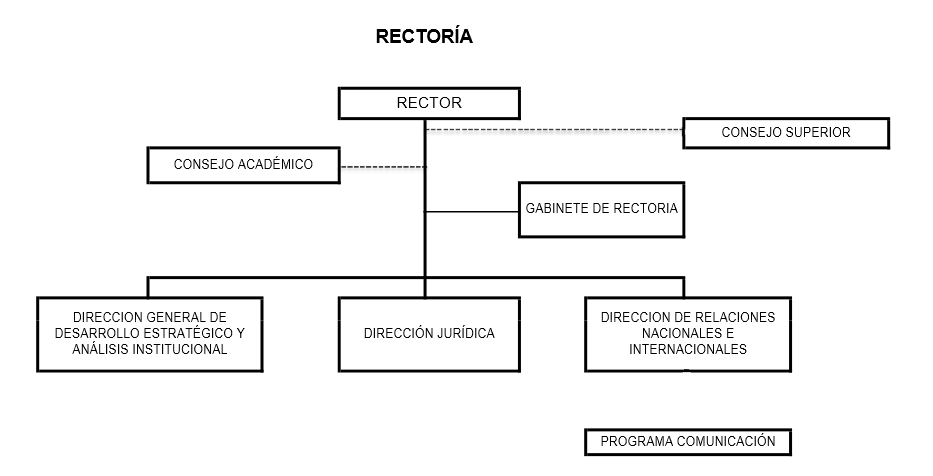
\includegraphics[scale=0.6,angle=0]{images/organigrama/1.png}
\caption{Organigrama de rector\'ia}
\label{Organigrama de rectoria}
\end{center}
\end{figure}

Es el segmento con mas poder en la organización universitaria, siendo este el foco central de las decisiones tomadas por los otros organismos. Es importante señalar que muchas de sus políticas provienen en gran medida de las necesidades y aspiraciones de las siguientes estructuras jerárquicas.

\subsection{Vicerrectoría Academica}
Es la entidad de que administra de manera local las decisiones de rectoría, hacia distintos polos como: Investigación, Dirección de evaluación, Dirección de docencia, Relaciones estudiantiles, Biblioteca, U.T.E.M. Virtual.
\begin{figure}[!hbp]
\begin{center}
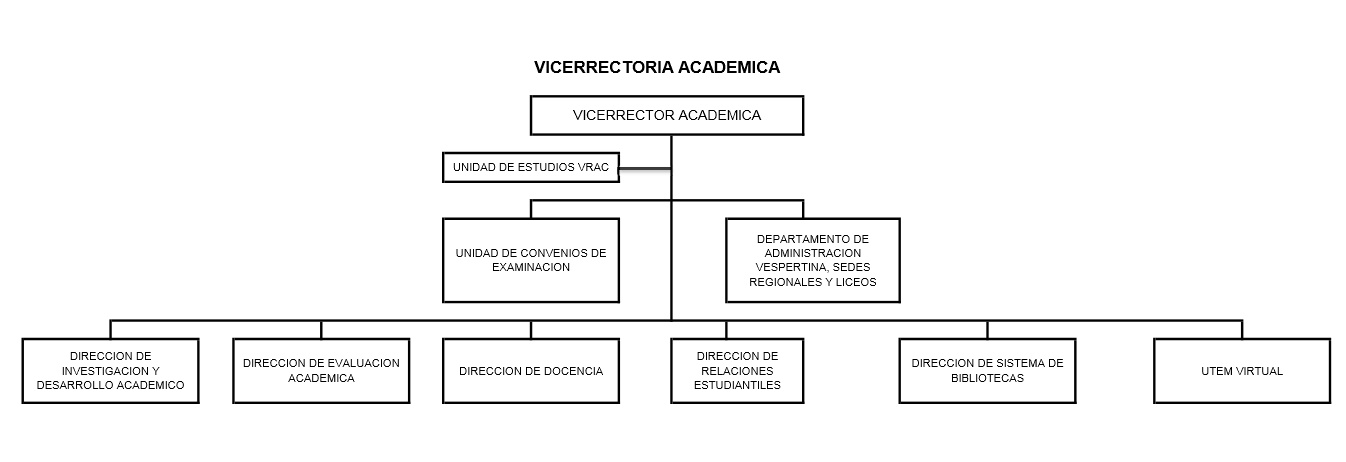
\includegraphics[scale=0.45,angle=0]{images/organigrama/2.png}
\caption{Organigrama de Vicerrector\'ia Academica}
\label{Organigrama de vicerrectoria Academica}
\end{center}
\end{figure}

Tiene el rol de velar por la correcta disponibilidad de recursos frente a los organismos de dirección institucional, para lo cual trabaja de manera constante en un perfeccionamiento de su rol como comandante.

\subsection{Facultad de ingeniería}
El decano de ingeniería es el principal responsable por las decisiones tomadas en esta estructura, debe liderar a todos los departamentos que le corresponden y cada uno de estos debe trabajar en pos de las directrices del decano de la facultad.
\begin{figure}[!hbp]
\begin{center}
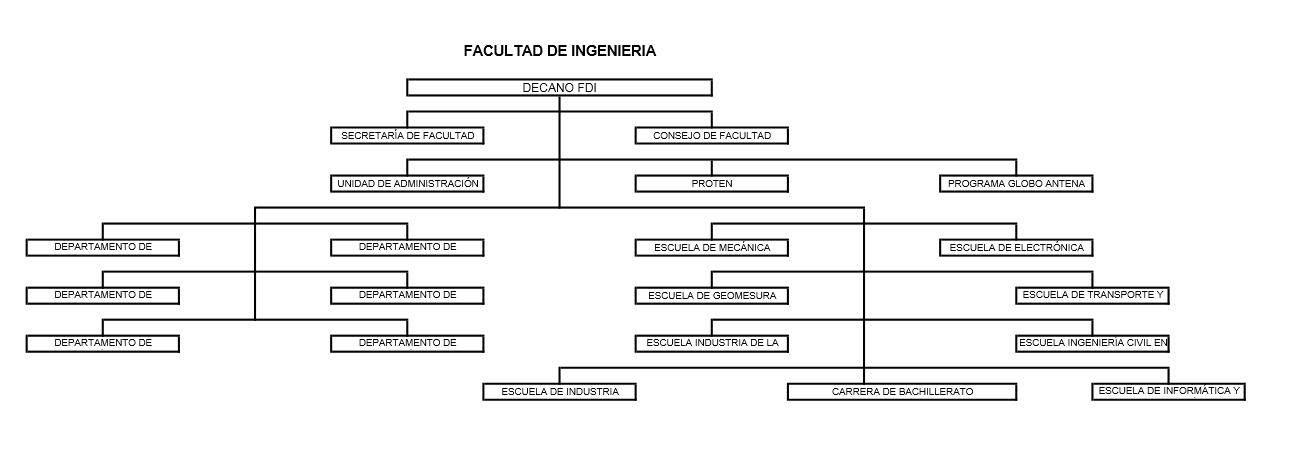
\includegraphics[scale=0.45,angle=0]{images/organigrama/11.png}
\caption{Organigrama de la facultad de ingen\'ieria}
\label{Organigrama de la facultad de ingenieria}
\end{center}
\end{figure}

\chapter{Problema}
\thispagestyle{empty}
\section{Situación Actual}
\subsection{Dirdoc}
El Dirdoc es una plataforma online en la que, alumnos, profesores y funcionarios tienen acceso, mediante distintos puntos de acceso, en cada uno de estos se ejecutan ciertas actividades. A continuación se detallan las características de cada uno.

\begin{itemize}
	\item Alumno: Es un acceso que le permite a un alumno mirar sus notas y sus promedios de todos sus ramos, además de la carrera, la maya curricular, entre otros.
	\item Profesor: Es un acceso en el que se permite la inserción de notas para los alumnos correspondientes, de acuerdo a los ramos que se imparten, entre otras cosas es posible mirar información del profesor, ramos en los que se trabaja y alumnos asociados a las clases.
	\item Funcionarios, son capaces de mirar información de todos los otros niveles, e incluso tienen facultades para editar información, para lo cual su uso esta centrado en regular el correcto funcionamiento de la herramienta DirDoc y tomar acciones frente a errores que puedan originarse.
\end{itemize}

\subsection{S.E.P.A.}
El S.E.P.A. (Sistema Estadístico de Profesores y Alumnos) es una herramienta complementaria en la U.T.E.M. que otorga principalmente indicadores estadísticos, que permiten tomar decisiones que afectan a un segmento importante de la organización. Por ejemplo se tiene el promedio de notas de un curso que imparte un profesor, o también el promedio de notas totales de un alumno. Si bien son importantes estos datos, pero son poco específicos.

Uno de los problemas que se tienen en sepa, es que al no existir un sistema de ingreso de data desde DirDoc, la única forma de ingresar data en sepa es mediante la petición a un funcionario encargado del sistema, lo que supone un riesgo por la perdida de data.

\section{Situación Propuesta}
Dentro de los módulos mantenedor e integrador de S.E.P.A. se comprenden las siguientes actividades que no están en la versión anterior:

\begin{itemize}
	\item Ingreso por perfiles: Gracias a las mejoras que se programan, se agrega el sistema de registro por perfiles, el cual otorga permisos por los distintos tipos de usuarios. Estos tendrán un rango de data que puedan visualizar. 
	\item Visualización de todas las tablas: En estas mejoras a S.E.P.A. se incorpora la posibilidad de mirar todos los parámetros de las tablas comprendidas en el modelo de base de datos. Esto significa que mediante los perfiles es posible ver la información historia de todas las tablas permitidas.
	\item Edición de todas las tablas: Como en el punto anterior, no solo es posible mirar, ya que también hay perfiles que pueden editar data de las tablas, pensando en la reparación de esta debido a que puede tener fallos o faltar.
	\item Integración por web service: El traspaso de data desde DirDoc a S.E.P.A. será mediante un servicio en linea de comunicación entre dos programas (DirDoc y S.E.P.A.), ya que de esta forma uno se asegura que la forma de ingreso de data en S.E.P.A. sea, en la mayor medida, limpia y sin errores. El sistema es capas de soportar la falta de ciertos datos en las tablas, los cuales pueden ser llenados posteriormente por el mantenedor que se incorpora.
	\item Facilidad de programar indicadores en un futuro: La forma de como esta programado S.E.P.A. supone una mejora, ya que al utilizar una tecnología que de rápido aprendizaje, es fácil encontrar otros desarrolladores que aporten con la programación de distintos indicadores. Ya que solo basta que se tenga gente con conocimientos específicos del entorno del servicio y la vista, sin conocer en detalle el modelo de la aplicación.
\end{itemize}
\section{Objetivos Generales y Específicos}
\subsection{Objetivos Generales}
\textit{Mejorar S.E.P.A. convirtiéndolo en un sistema de mantención de información estadística para la Universidad Tecnológica Metropolitana ayudando a sus procesos docentes y productivos, disponiendo de información veraz de la realidad universitaria.}

A partir de la versión actual de S.E.P.A., crear un sistema web basado en el patrón Modelo Vista Controlador, asegurando un producto que sea eficiente en el cumplimiento de sus objetivos. Las características principales serán que este sistema estará hecho en Java lo que nos permite una fácil implementación de las mejores prácticas de programación. Potenciando su valor en el tiempo, convirtiéndose en una herramienta cada ves mas útil y necesaria para el desarrollo de la organización.

\subsection{Objetivos Específicos}
\begin{enumerate}
	\item Generar un sistema que sea fácilmente mejorable, usando tecnologías estandarizadas y óptimas. Mediante JavaEE (Java Enterprise Edition), lo cual permite la integración de herramientas robustas dentro del software, tales como un sistema de mapeo de bases de datos a objetos simples de ocupar, un servicio web de comunicación entre dos sistemas, una vista con elementos de fácil interacción con el usuario final, entre otros.
	\item Entregar un producto de calidad, escalable y fiable para la comunidad universitaria. El cual sea un aporte para la toma de decisiones y también un soporte en la búsqueda de patrones o mejoras administrativas.
	\item Otro objetivo es la utilización de una metodología de desarrollo, en este caso PSP (Personal Software Process), la cual nos permite llevar un seguimiento y retroalimentación de las actividades que se deben realizar, de manera lógica y ordenada, para este propósito la metodología propone la utilización de valores contables en el tiempo, estos valores establecen las características y condiciones del trabajo del ingeniero. Lo cual entrega valor agregado al producto, mostrando data numérica y estadística del tiempo invertido en el trabajo y como este se va completando con eficiencia.
	\item Hacer una mejora sustancial en S.E.P.A. de manera que todo su conjunto sea útil para todos los usuarios a los que se enfoca, haciendo especial énfasis en que los perfiles a los que esta dirigido este trabajo puedan certificar mejoras en la calidad de la data, la rapidez del servicio, la seguridad que tiene, entre otras mejoras.  
	\item Producir una herramienta lo mas puramente moderna, que cumpla con calidad el objetivo propuesto, siendo un desafío para el desarrollador, incorporando herramientas simples que hacen el producto robusto y confiable, sin comprometer la facilidad de desarrollo futuro.
\end{enumerate}
%\chapter{Alcances y Limitaciones}
%\thispagestyle{empty}
%\section{Alcances del Proyecto}
%La coparticipación de indicadores UTIGRA (Unidad de Títulos y Grados) para trabajar con información pertinente a %gente que ha terminado sus procesos estudiantiles en la UTEM.

%Se crearan una serie de nuevos perfiles, y cada uno de estos tendrán su nivel de alcance en el sistema.
%\section{Limitaciones del Proyecto}
%El proyecto no contendrá requerimientos que se hagan fuera de lo requerido por el profesor como actividades de %Trabajo de Título.
%\section{Alcances del Trabajo de Título}
%Los alcances del Trabajo de Título están delimitados por las características que el trabajo de título debe tener, es %decir, que se hace un marco de trabajo, delimitado por el profesor, que comprende los tópicos a trabajar.
%\section{Limitaciones del Trabajo de Título}
%El trabajo no comprende áreas que estén fuera de los límites temporales a la toma de requerimientos, por lo cual es %necesario indicar que hay características y funcionalidades que a pesar de ser levantadas puede que no sean parte de %este trabajo de título.
\section{Estructura de desarrollo el proyecto}
El desarrollo del proyecto esta bajo la metodología Personal Sofware Process (PSP), la cual permite medir en forma cuantitativa todas la variables implicadas en el proceso productivo de este proyecto, lo que brindará valiosa información tanto del proyecto como del alumno.

Primero se crean una serie de tablas que registran el tiempo de desarrollo, la cantidad trabajada, y el porcentaje de avance, desde distintos puntos de vista, tales como: el desempeño diario, la cantidad de errores diarios, el avance semanal.

Después Se acomoda el tiempo en distintos indicadores que registran la cantidad de horas dedicadas el trabajo, ya sea en desarrollo como en estudio, sin olvidar el tiempo de descanso que se plantea. Este enfoque permite organizar el tiempo de acuerdo a actividades en función de completar el proyecto y la documentación PSP.

Finalmente se termina el proyecto y se tienen tablas completadas que muestran indicadores porcentuales de desempeño, cada ves mas eficiente y errores, cada ves mas tenues, lo que indica un avance generalizado y paulatino de la calidad en el proceso de desarrollo.
\chapter{Marco Teórico}
\thispagestyle{empty}
\section{Base Conceptual}
\subsection{Establecer el problema}
En la Universidad existe la necesidad de disponer de información relevante para apoyar la toma de decisiones, esta información debe ser respaldada por enormes volúmenes de registros que se guardan constantemente en el sistema DirDoc de la Universidad. Para este propósito existe el Sistema Estadístico de Profesores y Alumnos (S.E.P.A.), el cual incluye indicadores que pueden ser usados para el estudio de la institución. Con el tiempo la cantidad de datos va en crecimiento, también crece la cantidad de información y la necesidad de actualizar y modificar las tablas de manera más rápida y sencilla.

A raíz de esto se generaron ciertos problemas que comprometen la integridad de la data y por tanto entorpecen el objetivo inicial de S.E.P.A., estos son:

\begin{enumerate}
	\item Inserción de data en S.E.P.A., mediante la planificación con funcionarios de la universidad, se solicita la inserción de data desde DirDoc hacia S.E.P.A., lo que origina muchos problemas, como el tiempo que se ocupa en este proceso, la fácil probabilidad de falla debido a un error humano en varios puntos del proceso.
	\item Consultas que pueden ser lentas: Debido a que el sistema anterior S.E.P.A. estaba construido con PHP, el cual es una herramienta flexible pero de compleja mantención. Se hace poco eficiente su uso a medida que la cantidad de data va creciendo.
	\item No existe un modulo de actualización de data: Lo que hace a S.E.P.A. una herramienta con algunas cosas que no se pudieron programar en su momento.
	\item No existe un mecanismo de diferenciación de usuarios. Haciendo este sistema un tanto inseguro, ya que no debiera existir la posibilidad de mirar toda la data, si no solo una parte, en relación a un perfil.
	\item Data corrupta o inexistente: Dado que en el paso del tiempo la data esta corrupta, poco actualizada o simplemente no existe. Y la necesidad de esto se hace urgente.
\end{enumerate}
\subsection{Establecer la solución}
La solución de este proyecto es la creación de varios servicios web que proveen datos que deben ser procesados y mantenidos en una base de datos local. Este sistema debe validad la integridad de los datos evitando perdida de registros. A continuación se desarrolla un Mantenedor de los datos que componen el sistema, en el cual es posible buscar registros, comprobar que estén correctos, y si no lo están poder modificarlos.
\subsection{Uso de Java}
Esta actualización es construida a través del compendio de tecnologías que engloba la convención JavaEE (Java Enterprise Edition), caracterizada por un enfoque estandarizado en el proceso productivo, lo que permite automatizar varios procesos y centrarnos en el proyecto. Esto facilita la construcción del proyecto de manera más estable y segura. Agregando valor al proyecto mediante la incorporación de distintas herramientas, explicadas en este documento, que posibilitan un desarrollo de calidad y mejorable en el futuro.
\subsection{Desuso de PHP}
Algunas tecnologías como PHP permiten crear la página de manera rápida e incorporar un framework de persistencia pero son difíciles de escalar y mantener.  Otros frameworks como Ruby on Rails podrían llevar a cabo esta tarea de mejor manera. Pero el punto frágil es su curva de aprendizaje que es bastante alta.

Esto nos lleva a tomar la decisión de abandonar PHP ya que lo que se busca es, una herramienta que tenga reusabilidad en la organización y capacidad de mejora, manteniendo la robustez y la simpleza.
% enfocar a las cosas que no se pueden haceren otros lenguajes.
\section{Ciclo de vida del Software}
\begin{enumerate}
\item Toma de requerimientos: Proceso que básicamente comprende 2 actividades, primero la toma de requerimientos en base al sistema S.E.P.A. anterior, segundo una serie de entrevistas para captar las historias de usuarios que posteriormente se convierten en requerimientos.
\item Análisis de requerimientos: Etapa en donde el profesor encargado discute con el alumno los requerimientos que deben realizarse, de acuerdo con las expectativas y las necesidades del equipo de trabajo.
\item Diseño de la solución: Proceso en donde se desarrolla el modelo de datos que debe soportar a los requerimientos, y las interfaces asociadas.
\item Diseño estructural: En este punto el alumno trabaja desarrollando el proyecto en coordinación con el profesor encargado y éste va revisando constantemente el avance, emitiendo calificaciones y aclaraciones.
\item Pruebas: Proceso por el cual el profesor encargado verifica la fiabilidad y calidad de los requerimientos ya resueltos.
\item Instalación: En este punto se produce la incorporación del sistema en su ambiente por defecto, lo que implica un término del proyecto, solo dentro del marco de Trabajo de Título para el alumno de este proyecto.
\end{enumerate}

Desde esta perspectiva cada componente que se le quiera agregar al proyecto, debe obligatoriamente partir desde el Análisis de requerimientos, pasando por un Diseño de la solución, para después llegar al Diseño estructural y Pruebas, para finalmente Instalar los cambios.

%imagen de como tiene que ser
\section{Estado del arte}
La calidad de datos que se obtienen en un establecimiento educacional, es de vital importancia para la planificación y desarrollo de sus actividades, ya que permiten una normal toma de decisiones que afectan el desarrollo de la institución, ya sea de forma docente como administrativa. 

Los estudios estadísticos son tambien importantes porque entregan retroalimentación y permiten una visión más clara de la realidad operativa.

Las instituciones educacionales que producen profesionales deben estar evaluadas por organismos preparados en auditar las características de su desempeño. Para estos efectos, existen organismos estatales que acreditan lo que cada Universidad propone, pero por otro lado existen entandares de calidad que son medidos por organismos extranjeros, para dar un sello de calidad, evaluando a partir de datos estadísticos  \cite{data1}.

En 2009 se abre el sitio QS Top Universities que hasta el día de hoy es un sitio altamente eficiente en evaluación a trabes de ránkings enfocados a entregar información a organismos y personas relacionadas con post-grados, MBA, estudios de ingeniería y negocios, desarrollando estadísticas de alto alcance en sitios web, eventos, guías y programas por Internet y finalmente entregando soluciones técnicas a otros organismos, tales como Universidades o empresas privadas, entre otras.

Sus datos manejan información de 41 países, entre los que están: Argentina, Ecuador, Japon, Singapur, Australia, Egipto. Su servicio es sin costo para todo el público y permite un tipo de suscripción gratuita para visualizar tablas comparativas de manera simple.

Permite hacer comparaciones por categorías varias, ya sea país, estado, ciudad y otras características internas de la Universidad como ponderaciones o prestaciones de alumnos, tales como cantidad de alumnos o la segregación por sexo o etnia en cada localidad.

Su objetivo es ser el principal sitio de ránkings de educación con visualización con alcances estadísticos y comparativos a quienes estén dentro de su sistema.

Una debilidad de este sistema es que solo hace comparaciones de carácter global y no se involucra en temas más finos sobre cada Universidad, solo tiene datos recopilados de otras investigaciones para completar este tema.

Es una empresa de tamaño mediano, con más de 150 empleados en oficinas de todo el mundo. También se realizan Tours en 70 ciudades en 39 países que permiten a más de 50.000 espectadores, los cuales buscan entrar a una Universidad  \cite{data2}.

El Ránking de Calidad de las Universidades Chilenas, es un trabajo realizado por AméricaEconomía Intelligence en el 2010, un sitio de ránking para instituciones educacionales en Chile, que utiliza ciertos criterios, como lo son la cantidad de investigaciones, o la masa de estudiantes que entran en cada Universidad.

%Algunos datos generales que se obtienen, son que la Universidad de Chile y la PUC, tienen diferencias muy pequeñas %en el campo de la investigación, para lo cual se mostró que la Universidad de Chile aporto con 1.329 papers %publicados, en cambio la PUC hizo un aporte total de 1.029 publicaciones.

Mucha de esta data estadística es recopilada a traves de encuestas enviadas a distintas Universidades y organismos de educación en Chile. Cada institución trabaja con esto, con el fin de captar publico que desea tomar una decisión en el mercado.

Este sistema da cuenta de una necesidad por parte de las Universidades, de ser más competitiva en el mercado universitario. Aumentando los esfuerzos por recibir más estudiantes, mostrando mejores profesores, alumnos e investigaciones.

La gran debilidad de este sistema es que no se muestran muchos criterios de comparación y tanto solo da una arista para comparar lo que resulta insuficiente para formarse una opinión global del sistema.

Finalmente se observa a las Universidades actuales buscando organismos extranjeros capaces de certificar las características de la educación que ofrecen, de esta manera muestran no solo una acreditación por un organismo chileno, sino también una necesidad de competir a nivel internacional \cite{data3}.

\section{Justificación del Trabajo de Título}
La U.T.E.M. requiere un sistema informático que agregue funcionalidades para el control de sus datos de manera simple y segura. En el anterior S.E.P.A. los datos eran extraídos directamente del DirDoc, dando la posibilidad de cometer errores de inserción graves. Con este nuevo sistema, ahora no solo hay una seguridad con los datos que son transferidos desde servicios web, sino que también implementa un Sistema de Autenticación, gracias a su sistema de perfiles de usuarios que limita el acceso en el sitio para más de 2 tipos de usuarios.

El avance gracias al servicio web es justificado con las siguientes mejoras que se tienen que hacer para que esta modificación se pueda realizar:

\begin{itemize}
	\item Sistema de comunicación desde DirDoc hacia S.E.P.A.: Programar distintas interfaces que entregan información a S.E.P.A., pasando por todos los requerimientos que se puedan originar, y dejando paso a futuras peticiones por parte de este sistema a DirDoc.
	\item Sistema de rastreo de data y corrección: Programar un mecanismo que detecte cuando se presenten problemas con la data, ya sea que venga corrupta o mal formada, convirtiéndola en data en blanco, para posteriormente poder ser reparada.
	\item Sistema de inserción de data a un modelo estructurado para funcionar con JPA: Generar un modelo de datos que permita la interacción frente al patrón Modelo, Vista, Controlador, en donde el modelo es la estructura simple de la data, pero permite tomar todos los conjuntos de data de manera fácil, rápida y óptima.
	\item Sistema cronométrico de petición de data a DirDoc: Programar un sistema que haga las distintas consultas a DirDoc de manera cronometrada, ocupando distintos horarios para hacer las ejecuciones. Por ejemplo haciendo que las ejecuciones sean en un horario en que poca gente hace uso de los servicios. Minimizando los recursos.
\end{itemize}

Por otro lado la creación del sistema mantenedor comprende las siguientes mejoras:

\begin{itemize}
	\item Inserción de perfiles de usuario: Programar por medio de herramientas dentro de JavaEE, distintos perfiles que serán capaces de mirar en ciertas medidas la data que ofrece el sistema.
	\item Mejora de la interfaz de usuario: Programar componentes que el usuario pueda aprender a usar de forma rápida y eficiente.
	\item Uso completo de las tablas de S.E.P.A.: Mediante los distintos perfiles es posible llegar a todas las tablas, lo que supone el mantenimiento de todas estas.
	\item Visualización y mantenimiento de las tablas: Programar sistema de mantenimiento para todas las tablas que un usuario pueda visualizar
\end{itemize}

\section{Análisis de las herramientas}
El desarrollo de las aplicaciones debe ser con un lenguaje que nos permita la correcta ejecución de las tareas de diseño y desarrollo. Por lo cual resulta interesante desarrollar algunos criterios que nos mostrarán las características y la justificación de nuestra elección a la hora de pensar en un lenguaje apropiado para este proyecto.

\begin{enumerate}

\item Sencillez: Característica del lenguaje que hace que sea fácil el crear o entender el código, al momento de programarlo o leerlo \cite{data4}.

\item Robustez: Capacidad interna del lenguaje de proporcionar herramientas que permiten minimizar los errores producidos por el programador \cite{data4}.

\item Seguridad: Característica que hace que un lenguaje no permita tocar accesos a donde la aplicación no debiese ir (en la mayoría de los casos), ejemplos como, restringir accesos, ejecución de pruebas o derechos de accesos \cite{data4}.

\item Portabilidad: Capacidad de un lenguaje para correr en múltiples sistemas operativos \cite{data4}.

\item Neutralidad: Independencia de la maquina en donde se ejecuta, concibiendo una experiencia lo más similar posible entre distintas máquinas y sistemas operativos \cite{data4}.

\item Interfaz: Capacidad de producir fácilmente interfaces cómodas para el usuario final \cite{data4}.

\item Expresividad: Capacidad de minimizar el número de líneas con las que una acción puede ejecutarse dentro del código \cite{data5}.

\item Compilación: Capacidad de minimizar el tiempo que toma poder compilar el código producido.

\item Aprendizaje: Dificultad para aprender el lenguaje. Basado simplemente en la experiencia propia sobre cada lenguaje.

\item Estructuras de control: Un lenguaje debe proveer estructuras simples de control, pero tampoco llenarse de estructuras que nunca se van a utilizar \cite{data6}.

\item Abstracción: Capacidad de convertir cosas difíciles en algo simple con la estructura del lenguaje \cite{data6}.

\end{enumerate}

También es importante tener en cuenta el lenguaje a utilizar en el momento de la creación del proyecto, de esta manera se pondrán los lenguajes candidatos para conocerlos en mayor detalle.

\begin{enumerate}

\item PHP: Es el lenguaje de lado servidor más extendido en la web. Surgido en 1994, se trata de un lenguaje de creación relativamente reciente, aunque con la rapidez con la que evoluciona Internet parezca que ha existido toda la vida. Es un lenguaje que ha tenido una gran aceptación en la comunidad de desarrolladores, debido a la potencia y simplicidad que lo caracterizan, así como al soporte generalizado en la mayoría de los servidores \cite{data7}.

\item .NET: Es un framework de Microsoft que hace un énfasis en la transparencia de redes, con independencia de plataforma de hardware y que permita un rápido desarrollo de aplicaciones. Basado en ella, la empresa intenta desarrollar una estrategia horizontal que integre todos sus productos, desde el sistema operativo hasta las herramientas de mercado \cite{data8}.

\item Ruby on Rails: Es un entorno de desarrollo web de código abierto que está optimizado para satisfacción de los programadores y de la productividad. Te permite escribir un buen código favoreciendo la convención antes que la configuración \cite{data9}.

\item Java: Es un lenguaje de programación de propósito general. En la actualidad es un lenguaje muy extendido y cada vez cobra más importancia tanto en el ámbito de Internet como en la informática en general. Está desarrollado por la compañía Oracle con gran dedicación y siempre enfocado a cubrir las necesidades tecnológicas de punta. \cite{data10}.
\end{enumerate}

En la siguiente tabla muestra una comparación de las cuatro tecnologías anteriormente presentadas de forma explicita para comprender nuestra elección. Es claro decir que uno de los aspectos que marca profundamente la elección sobre el lenguaje con que se va a realizar este proyecto, es determinada por los conocimientos que tiene el alumno y las indicaciones del profesor, en pos de realizar lo más rápido posible el trabajo, haciéndolo de forma elegante. 

\begin{tabular}{| l | l | l | l | l |}
\hline
 & 
\includegraphics[scale=0.08]{images/icons/php.png} & 
\includegraphics[scale=0.08]{images/icons/net.png} & 
\includegraphics[scale=0.51]{images/icons/ruby-on-rails.png} & 
\includegraphics[scale=0.1]{images/icons/java.png}\\
\hline
\textit{Sencillez} & \textcolor{green}{\CheckmarkBold} &  \textcolor{red}{\XSolidBold} &  \textcolor{red}{\XSolidBold} & \textcolor{green}{\CheckmarkBold}\\
\hline
\textit{Robustez} & \textcolor{red}{\XSolidBold} & \textcolor{green}{\CheckmarkBold} & \textcolor{green}{\CheckmarkBold} & \textcolor{green}{\CheckmarkBold}\\
\hline
\textit{Seguridad} & \textcolor{red}{\XSolidBold} & \textcolor{red}{\XSolidBold} & \textcolor{green}{\CheckmarkBold} & \textcolor{green}{\CheckmarkBold}\\
\hline
\textit{Portabilidad} & \textcolor{green}{\CheckmarkBold} & \textcolor{red}{\XSolidBold} & \textcolor{red}{\XSolidBold} & \textcolor{green}{\CheckmarkBold}\\
\hline
\textit{Neutralidad} & \textcolor{green}{\CheckmarkBold} & \textcolor{red}{\XSolidBold} & \textcolor{green}{\CheckmarkBold} & \textcolor{green}{\CheckmarkBold}\\
\hline
\textit{Interfaz} & \textcolor{red}{\XSolidBold} & \textcolor{green}{\CheckmarkBold} & \textcolor{green}{\CheckmarkBold} & \textcolor{green}{\CheckmarkBold}\\
\hline
\textit{Expresividad} & \textcolor{green}{\CheckmarkBold} & \textcolor{red}{\XSolidBold} & \textcolor{green}{\CheckmarkBold} & \textcolor{red}{\XSolidBold}\\
\hline
\textit{Compilación} & \textcolor{green}{\CheckmarkBold} & \textcolor{red}{\XSolidBold} & \textcolor{green}{\CheckmarkBold} & \textcolor{red}{\XSolidBold}\\
\hline
\textit{Aprendizaje} & \textcolor{green}{\CheckmarkBold} & \textcolor{red}{\XSolidBold} & \textcolor{green}{\CheckmarkBold} & \textcolor{green}{\CheckmarkBold}\\
\hline
\textit{E. de control} & \textcolor{green}{\CheckmarkBold} & \textcolor{green}{\CheckmarkBold} & \textcolor{green}{\CheckmarkBold} & \textcolor{green}{\CheckmarkBold}\\
\hline
\textit{Abstracción} & \textcolor{green}{\CheckmarkBold} & \textcolor{red}{\XSolidBold} & \textcolor{red}{\XSolidBold} & \textcolor{green}{\CheckmarkBold}\\
\hline
\textbf{Total} & 8 & 3 & 8 & 9\\
\hline
\end{tabular}

Como lo muestra la tabla anterior, java es el que puede cumplir más criterios, en el sentido de la observación y el criterio subjetivo del alumno que realiza el trabajo.

\section{Criterios de Calidad}

Se mostrarán a continuación los criterios de calidad del proyecto. Estos criterios muestran de forma justificada, que la mejor elección es la que nosotros proponemos para la organización, pensando en los costes de tiempo y recursos económicos que un proyecto de esta clase puede significar.

\begin{enumerate}

\item Mantenibilidad: Característica que hace que nuestro proyecto sea fácil de corregir en caso de fallos. Basándose en la concepción de que un proyecto que tiene un modelo bien establecido es más fácil de reparar \cite{data11}.

\item Flexibilidad: Característica que indica la capacidad de agregar cambios, incluyendo también el hecho de que como es un sistema hecho dentro del contexto de esta Universidad está lo suficientemente enfocado en ella, pero también es posible cambiar algunas cosas en pos de que este sistema funcione también en otras Universidades. \cite{data11}.

\item Testeabilidad: Esto nos muestra que el modelo del sistema ha pasado por un test antes de ser ocupado en el proyecto. \cite{data11}.

\item Portabilidad: Ya que como se trabaja con Java, el proyecto es básicamente portable a casi cualquier tipo de sistema operativo, lo que lo hace un ente fácil de cambiar en otros entornos de trabajo y es perfectamente acomodable en ese sentido. \cite{data11}.

\item Integridad: Este sistema se caracteriza por su integridad con los datos, lo que nos muestra un dedicado trabajo sobre el tema de la base de datos. \cite{data11}.

\item Rapidez: El sistema está hecho de tal manera que debe funcionar de forma expedita y veloz, sobre todo con la enorme cantidad de datos que se van a manejar. \cite{data11}.

\end{enumerate}

\section{Patrones de Diseño}
Son arquitecturas estandarizadas para el desarrollo de software, permiten a los proyectos ser resueltos con estrategias ya probadas y que funcionan en la mayoría de los casos. Existen muchos patrones distintos, algunos de ellos son:

\begin{enumerate}

\item MVC, Modelo Vista Controlador: Establece que el software tiene por lo menos 3 capas de desarrollo las cuales son; modelo, donde se encuentran el acceso a datos como de una base de datos, ficheros o servicio web; vista, la parte del programa que interactúa con el usuario final; controlador, el código en donde esta el negocio que procesa los datos del modelo para posteriormente mostrarlos en la vista.

\item SOA, Arquitectura orientada a servicios: Establece el software enfocado a los procesos de negocio, teniendo distintas capas de aplicaciones como: Aplicaciones básicas, caracterizadas por ser pequeñas y geográficamente establecidas; Exposición de Funcionalidades, donde rigen servicios; Integración de servicios, para intercambio de datos; Composición de procesos, determina términos de negocio y funcionalidades; Entrega, para usuarios finales.

\item POA, Programación Orientada al Aspecto: Es un paradigma de programación relativamente reciente cuya intención es permitir una adecuada modularización de las aplicaciones y posibilitar una mejor separación de incumbencias. Con esto se pueden encapsular los diferentes conceptos que componen una aplicación en entidades bien definidas, eliminando las dependencias entre cada uno de los módulos. De esta forma se consigue razonar mejor sobre los conceptos, se elimina la dispersión del código y las implementaciones resultan más comprensibles, adaptables y reusables.

\item DAO, Objeto de Acceso a datos: es un componente de software que suministra una interfaz común entre la aplicación y uno o más dispositivos de almacenamiento de datos, tales como una Base de datos o un archivo. El término se aplica frecuentemente al Patrón de diseño Object. Los Objetos de Acceso a Datos son un Patrón de los subordinados de Diseño Core J2EE y considerados una buena práctica. La ventaja de usar objetos de acceso a datos es que cualquier objeto de negocio (aquel que contiene detalles específicos de operación o aplicación) no requiere conocimiento directo del destino final de la información que manipula.

\end{enumerate}

\chapter{Introducción al PSP}
\thispagestyle{empty}
\section{Base teórica}
PSP (Proceso de Software Personal) es una metodología de desarrollo para proyectos informáticos, que tiene una serie de pasos enfocados en el ordenamiento, cuantificación y la categorización del trabajo y el tiempo. Es usada mundialmente por su fácil aprendizaje y su rápida incorporación. Este modelo de trabajo es solo para proyectos personales, o sea, en donde el desarrollador toma todo el trabajo por sí solo.

Este tipo de trabajo nos proporciona una serie de tablas que muestran nuestros tiempos de desarrollo y avance del proyecto, básicamente en el PSP nosotros podemos obtener los tiempos de desarrollo y la cantidad de líneas de código para cada actividad o conjunto de actividades. De esta manera uno puede llegar a determinar un factor de calidad dentro de nuestro trabajo dentro de los estándares que uno estime conveniente utilizar.

PSP nos obliga a desarrollar una forma de trabajo en la cual un desarrollador programa y anota los tiempos de desarrollo y la cantidad de código que uno ha producido, dentro de distintas tablas hechas para ese propósito.

\section{Criterios para uso de PSP}
La necesidad de usar PSP fue concebida para generar un proyecto que tuviera un criterio de calidad cuantificable. Ya que nos proporcionaba tablas e indicadores que establecen con el tiempo empleado, la cantidad de esfuerzo y errores que uno puede cometer en el trascurso del proyecto.

\section{Estructura del PSP}
\subsection{El trabajo del ingeniero de sofware}
En este apartado se listan las actividades que contemplan el desarrollo del proyecto, incluyendo todo lo que pueda servir como avances en el proyecto, ya sea investigar, reunirse con otros o desarrollar.
\subsection{La gestión del tiempo}
Para este punto solo se necesita la estructuración del tiempo que uno tiene sobre el tiempo que se pretende dar al proyecto, basándose en la lista de actividades.
\subsection{El control del tiempo}
Para este apartado se desarrolla una tabla que contiene una lista de actividades con los tiempos de inicio y término de cada una de las tareas que se hacen. También se anotan los tiempos perdidos, el tipo de actividad y si está completada o no.
\subsection{Planificación de períodos y productos}
Este apartado se preocupa de la planificación semanal del tiempo, en la parte de desarrollo se tienen 3 tablas que nos permiten llevar los registros totales de tiempo en minutos de las actividades hecha durante la semana. La primera tabla muestra las sumas de los tiempos, la segunda muestra la actividad de las semanas pasadas y la tercera muestra el total de las semanas hasta hoy en día.
\subsection{La planificación del producto}
El desarrollo del proyecto requiere de un cuaderno que registre la actividad en función de los trabajos que se van realizando, para lo cual se tiene un cuaderno de trabajos que registra las actividades con sus respectivas estimaciones de tiempo, sacadas de datos anteriores. Recordar que en esta tabla se anotan los trabajos que resumen las actividades diarias, así que se anota uno al día.
\subsection{El tamaño del producto}
Para estimar los costes de tiempo y valor de cada actividad que representa parte del desarrollo del un producto como tal, es necesario establecer formas de medición para valores que pueden ser cuantificables en unidades de trabajo. Para lo cual en esta actividad se mostrarán Estimaciones de Tamaños para las actividades particulares de este proyecto.
\subsection{La gestión del tiempo}
Para poder desarrollar las actividades, se necesita tiempo, por lo cual resulta importante manejarlo apropiadamente, para esto se hace una estimación aproximada del tiempo que consumirá la ejecución de las actividades relacionadas con el desarrollo del trabajo que está en curso. Se expondrán dos tablas y un marco de referencias para las aproximaciones futuras.
\subsection{La gestión de los compromisos}
Los compromisos que uno hace con las personas a las cuales espera entregar un proyecto, deben ser documentados, mostrando el tipo de actividad a realizar, el día, los participantes de ese compromiso, la hora en que se realiza, la fecha y finalmente lo que se recibe a cambio de la finalización de estas tareas. Es importante destacar que una correcta forma de manejar los compromisos lleva a un buen plan de trabajo.
\subsection{La gestión de las programaciones}
En un proyecto siempre es necesario definir las características importantes que comprenden la ejecución de cada una de las actividades que se están desarrollando, por tanto en este proyecto se tiene un registro de los puntos de control, los cuales representan las características importantes que el desarrollo de este trabajo debe comprender.
\subsection{El plan del proyecto}
Para generar un plan del proyecto se necesita tener un resumen de las características de cómo se desarrolla el trabajo, para lo cual se expondrá un molde para generar planes de proyectos, mediante el cual se estima la cantidad de esfuerzo que uno puede desarrollar de acuerdo a las labores anteriores que ha realizado. Finalmente se mostrará un ejemplo de estimación del tamaño del programa.
\subsection{Defectos}
El registro de los defectos es altamente importante, ya que nos permite la correcta verificación de cada incidente ocurrido dentro del proceso de desarrollo del software. El cuaderno de registro de errores se ocupa en el desarrollo de aplicaciones, y nos permite anotar un error cuando ha salido en modo de compilación para lo cual uno registra el tipo de error y el tiempo dedicado a la reparación de este error. El objetivo de esta tabla es impedir la repetición de ciertos errores que pueden ser reparados mediante el aprendizaje.\\
\\
\textbf{Tipos de Defectos}\\
\begin{tabular}{| l | l | l | l |}
\hline
10 & Documentación         & 60 & Comprobación\\
\hline
20 & Sintaxis              & 70 & Datos\\
\hline
30 & Construcción Paquetes & 80 & Función\\
\hline
40 & Asignación            & 90 & Sistema\\
\hline
50 & Interfaz              & 100 & Entorno\\
\hline
\end{tabular}

\chapter{Aplicación del PSP}
\thispagestyle{empty}
\section{Explicación}
Se mostrará la forma de desarrollo de las tablas PSP más importantes en el proyecto dando cuenta de cómo es el desempeño del PSP dentro de nuestro proyecto S.E.P.A.. Tendremos el desarrollo de las tablas más importantes en el PSP frente a nuestra operación. Obtendremos una mirada clara frente a que es el PSP y como éste permite complementar calidad en nuestra ocupación.
\section{Desarrollo del PSP}
\subsection{El Trabajo del Ingeniero de Sofware}
Para estos efectos se desarrollo la siguiente tabla de actividades, con su frecuencia semanal y sus minutos.

\begin{tabular}{|l | l | l |}
\hline
\textbf{Tarea} & \textbf{Frecuencia (semanal)} & \textbf{Tiempo (minutos)} \\
\hline
Estudiar documentos & todos & 840/semana\\
\hline
Desarrollo & todos & 1260\\
\hline
Programar & todos & 2520\\
\hline
Reuniones & L, M, J & 420/semana\\
\hline
Reparar Documentos & Mi, V & 840/semana\\
\hline
\end{tabular}
\subsection{La Gestión del Tiempo}
En este caso en particular uno puede ver que se tienen todos los días de la semana destinados para el propósito de desarrollar el proyecto ya sea en informes o programar. En menos tiempo se reparten las tareas de investigar y reparar cosas.
\subsection{El Control del Tiempo}
Se muestra la siguiente tabla de control de Tiempo, de forma resumida, para un día en especifico.

\begin{tabbing}
Estudiante: \= Miguel Angel Fuenzaldia Pino \= Fecha: \= 9/10/2012\\
Profesor: \> Sebastián Salazar Molina \>   \>  \\
\end{tabbing}
\begin{tabular}{| l | l | l | l | l | l | l | l | l |}
\hline
\textbf{Fecha} & \textbf{Comienzo} & \textbf{Fin} & \textbf{Delta} & \textbf{Actividad} & \textbf{Comentarios}\\
\hline
19/11 & 10:56 & 11:17 & 20 & Desarrollo & notebook\\
\hline
      & 11:18 & 11:35 & 15 & lectura & psp\\
\hline
      & 11:35 & 12:29 & 50 & Desarrollo & notebook\\
\hline
      & 12:30 & 12:56 & 30 & lectura & psp\\
\hline
      & 12:57 & 13:02 & 5 & Desarrollo & notebook\\
\hline
      & 13:02 & 13:29 & 30 & Almorzar & olgura\\
\hline
      & 13:30 & 15:21 & 120 & Desarrollo & notebook\\
\hline
      & 15:22 & 16:12 & 45 & lectura & psp\\
\hline
      & 15:22 & 16:00 & 40 & Desarrollo & notebook\\
\hline   
20/11 & 16:00 & 17:00 & 60 & Desarrollo & notebook\\
\hline
      & 17:00 & 18:26 & 90 & lectura & psp\\
\hline
      & 18:30 & 19:00 & 30 & Desarrollo & notebook\\
\hline 
21/11 & 18:00 & 18:30 & 30 & lectura & psp\\
\hline
      & 18:30 & 19:00 & 30 & Desarrollo & notebook\\
\hline 
26/11 & 15:00 & ... & ... & Desarrollo & notebook\\
\hline
\end{tabular}
\subsection{Planificación de Períodos y Productos}
Se muestran las siguientes tablas de planificación, de forma resumida, para comprender como se utilizan.

\textbf{Estudiante}: Miguel Angel Fuenzaldia Pino     \textbf{Fecha}: 9/10/2012\\
\begin{tabular}{| l | l | l | l | l | l |}
\hline
\textbf{Tarea} & \textbf{Reunion} & \textbf{Codificar} & \textbf{Escribir} & \textbf{Leer} & \textbf{Total} \\
\hline
\textbf{Fecha} &                  & \textbf{Programas} & \textbf{Textos} & \textbf{textos} & \\
\hline
D 18/11 & & & & & \\
\hline
L & & 180 & 60 & 60 & 350\\
\hline
M & & & & & \\
\hline
Mi & & 180 & 60 & 60 & 350\\
\hline
J & 120 & & & & 120\\
\hline
V & & 180 & 60 & 60 & 350\\
\hline
S & & & & & \\
\hline
\textbf{Totales} & 120 & 540 & 180 & 180 & 1170\\
\hline
\end{tabular}
\\
Tiempos y Medias del Período, Número de Semanas (número anterior +1): 1\\
Resumen de las semanas anteriores:\\
\begin{tabular}{| l | l | l | l | l | l |}
\hline
\textbf{Total} & 1170 & 1290 & 1170 & 1150 & 1170 \\
\hline
\textbf{Med.} & 1000 & 900 & 500 & 1000 & 1000 \\
\hline
\textbf{Máx} & 1170 & 1290 & 1170 & 1150 & 1170 \\
\hline
\textbf{Mín} & 900 & 800 & 400 & 900 & 800 \\
\hline
\end{tabular}
\\
Resumen de las semanas totales (anteriores mas última)\\
\begin{tabular}{| l | l | l | l | l | l |}
\hline
\textbf{Total} & 1170 & 2460 & 3630 & 4780 & 5950 \\
\hline
\textbf{Med.} & 1000 & 1900 & 2400 & 3400 & 4400 \\
\hline
\textbf{Máx} & 1170 & 2460 & 3630 & 4780 & 5950 \\
\hline
\textbf{Mín} & 900 & 1700 & 2100 & 3000 & 3800 \\
\hline
\end{tabular}
\subsection{La Planificación del Producto}
La siguiente tabla muestra una forma de planificación.

\textbf{Estudiante}: Miguel Angel Fuenzaldia Pino     \textbf{Fecha}: 9/10/2012\\
\begin{tabular}{|c|c|c|c|c|c|c|c|c|c|c|c|c|}
\hline
\textbf{Trab} & \textbf{Fecha} & \textbf{Pro} & \multicolumn{2}{|c|}{\textbf{Estimado}} & \multicolumn{3}{|c|}{\textbf{Real}} & \multicolumn{5}{|c|}{\textbf{Hasta la Fecha}} \\
\hline
 & & & \textbf{Tie} & \textbf{Uni} & \textbf{Tie} & \textbf{Uni} & \textbf{Vel} & \textbf{Tie} & \textbf{Uni} & \textbf{Vel} & \textbf{Máx} & \textbf{Mín} \\
\hline
\multirow{2}{*}{1} & 19/11 & Escr. & 420 & 1 & 300 & 2 & 150 & 300 & 2 & 150 & 150 & 150 \\
\cline{2-13} & \multicolumn{12}{|l|}{\textbf{Descripción:} Escribir el Engineer Notebook para los capitulos 5 al 12}\\
\hline
\multirow{2}{*}{2} & 20/11 & Escr. & 420 & 1 & 300 & 2 & 150 & 300 & 2 & 150 & 150 & 150 \\
\cline{2-13} & \multicolumn{12}{|l|}{\textbf{Descripción:} Escribir el Engineer Notebook para los capitulos 7 al 16}\\
\hline
\multirow{2}{*}{n} & & & & & & & & & & & & \\
\cline{2-13} & \multicolumn{12}{|l|}{\textbf{Descripción:}}\\
\hline
\end{tabular}
\subsection{El Tamaño del Producto}
Se tiene una muestra de tablas por actividad para determinar la cantidad total de trabajo que se realiza con respecto a lo que se tiene que tener al final.

\begin{tabbing}
\textbf{Estudiante:} \= Miguel Angel Fuenzaldia Pino \= \textbf{Fecha:} \= 19/11/2012\\
\textbf{Profesor:} \> Sebastián Salazar Molina \> \textbf{Tiempos de Actividad} \>  \\
\end{tabbing}
\textbf{Reunión}\\
\begin{tabular}{| l | l | l | l |}
\hline
\textbf{Persona} & \textbf{Tiempo} & \textbf{Temas} & \textbf{Tiempo x Tema}\\
\hline
Sebastián Salazar & 60 & 4 & 15\\
\hline
\textbf{Totales} & 60 & 4 & 15 \\
\hline
\textbf{Medias} & 60 & 4 & 15 \\
\hline
\end{tabular}
\\\\
\textbf{Lectura}\\
\begin{tabular}{| l | l | l | l |}
\hline
\textbf{Capítulo} & \textbf{Tiempo} & \textbf{Páginas} & \textbf{Tiempo x Página}\\
\hline
1-5   & 180 & 50 & 3,6 \\
\hline
6-10  & & & \\
\hline
11-15 & & & \\
\hline
16-20 & & & \\
\hline
\textbf{Totales} & 180 & 50 & 3,6 \\
\hline
\textbf{Medias} & 180 & 50 & 3,6 \\
\hline
\end{tabular}
\\\\
\textbf{Escribir}\\
\begin{tabular}{| l | l | l | l |}
\hline
\textbf{Documento} & \textbf{Tiempo} & \textbf{Páginas} & \textbf{Tiempo x Página}\\
\hline
PSP & 360 & 30 & 20 \\
\hline
Bitácora & 10 & 1 & 10 \\
\hline
Título & & & \\
\hline
\textbf{Totales} & 370 & 31 & 30 \\
\hline
\textbf{Medias} & 185 & 15,5 & 15 \\
\hline
\end{tabular}
\\\\
\textbf{Programar}\\
\begin{tabular}{| l | l | l | l | l | l | l |}
\hline
\textbf{Programa} & \textbf{LOC} & \textbf{Func. Anteriores} & \textbf{Func. Hasta} & \textbf{Mín} & \textbf{Media} & \textbf{Máx}\\
\hline
Modelo & 			500  & 400 & 200 & 200 & 400 & 500 \\
\hline
Control &			100  & 50  & 25  & 25  & 50  & 100 \\
\hline
Vista &  			400  & 350 & 175 & 175 & 350 & 400\\
\hline
\textbf{Totales} &	1000 & 800 & 200 & 200 & 800 & 1000 \\
\hline
\textbf{Medias} & 	500	 & 400 & 100 & 100 & 400 & 500\\
\hline
\end{tabular}
\subsection{La Gestión del Tiempo}
Se muestran las tablas de gestión del tiempo por actividades.

\begin{tabbing}
\textbf{Estudiante:} \= Miguel Angel Fuenzaldia Pino \= \textbf{Fecha:} \= 19/11/2012\\
\textbf{Profesor:} \> Sebastián Salazar Molina \> \textbf{Tiempos de Actividad} \>  \\
\end{tabbing}
\textbf{Toma de Requerimientos y Preparación de Engineer Notebook}\\
\begin{tabular}{| l | l | l | l | l | l |}
\hline
\textbf{Tarea} & \textbf{Reunion} & \textbf{Codificar} & \textbf{Escribir} & \textbf{Leer} & \textbf{Total} \\
\hline
\textbf{Fecha} &                  & \textbf{Programas} & \textbf{Textos} & \textbf{textos} & \\
\hline
D  &    & & 180 & 180 & 360 \\
\hline
L  & 60 & & 180 & 180 & 420 \\
\hline
M  &    & & 180 & 180 & 360 \\
\hline
Mi & 60 & & 180 & 180 & 420 \\
\hline
J  &    & & 180 & 180 & 360 \\
\hline
V  & 60 & & 180 & 180 & 420 \\
\hline
S  &    & & 180 & 180 & 360 \\
\hline
\textbf{Totales} & 180 & & 1260 & 1260 & 1440 \\
\hline
\end{tabular}
\\\\
\textbf{Etapa de desarrollo de Proyecto e Informe}\\
\begin{tabular}{| l | l | l | l | l | l |}
\hline
\textbf{Tarea} & \textbf{Reunion} & \textbf{Codificar} & \textbf{Escribir} & \textbf{Leer} & \textbf{Total} \\
\hline
\textbf{Fecha} &                  & \textbf{Programas} & \textbf{Textos} & \textbf{textos} & \\
\hline
D  &    & 180 & 180 &  & 360 \\
\hline
L  & 60 & 180 & 180 &  & 420 \\
\hline
M  &    & 180 & 180 &  & 360 \\
\hline
Mi & 60 & 180 & 180 &  & 420 \\
\hline
J  &    & 180 & 180 &  & 360 \\
\hline
V  & 60 & 180 & 180 &  & 420 \\
\hline
S  &    & 180 & 180 &  & 360 \\
\hline
\textbf{Totales} & 180 & 1260 & 1260 &  & 2700 \\
\hline
\end{tabular}
\subsection{La Gestión de los Compromisos}
La siguiente tabla muestra un ejemplo de los compromisos y la información de acuerdo a cada tarea que uno pretende realizar.

\begin{tabbing}
\textbf{Estudiante:} \= Miguel Angel Fuenzaldia Pino \= \textbf{Fecha:} \= 19/11/2012\\
\textbf{Profesor:} \> Sebastián Salazar Molina \> \textbf{Tiempos de Actividad} \>  \\
\end{tabbing}
\textbf{Lista de Compromisos}\\
\begin{tabular}{| l | l | l | l | l | l |}
\hline
\textbf{Fecha} & \textbf{Compromizo} & \textbf{¿Con quíen?} & \textbf{Horas} & \textbf{Fin} & \textbf{Consigo} \\
\hline
D  & Leer       & Propio   & 3 & Dom & Conocimiento \\
\hline
L  & Desarrollo & Cliente  & 3 & ... & Título \\
\hline
M  & Escribir   & Profesor & 3 & ... & Título \\
\hline
Mi & Desarrollo & Cliente  & 3 & ... & Título \\
\hline
J  & Reunión    & Profesor & 1 & ... & Información \\
\hline
V  & Desarrollo & Cliente  & 3 & ... & título \\
\hline
S  & Escribir   & Profesor & 3 & ... & título \\
\hline
\end{tabular}
\subsection{La Gestión de las Programaciones}
A continuación una tabla que muestra un poco como una persona que utiliza el PSP puede programar su lista de actividades.

\textbf{Estudiante}: Miguel Angel Fuenzaldia Pino     \textbf{Fecha}: 9/10/2012\\\\\
\begin{tabular}{| l | l |}
\hline
\multicolumn{2}{|c|}{\textbf{Puntos de Control}}\\
\hline
\textbf{Numero} & \textbf{Punto de Control}\\
\hline
1 & Desarrollar el Cuaderno de Anotaciones para la Metodología PSP \\
\hline
2 & Asistir a reuniones con el profesor encargado del ramo \\
\hline
3 & Desarrollar el Sofware que se pide, a traves de los requerimientos conseguidos \\
\hline
4 & Escribir un informe de título en coordinación con lo requerido\\
\hline
\end{tabular}
\subsection{El Plan del Proyecto}
Se tiene un molde de lo que es el plan del proyecto, que es la parte más consistente del desarrollo en PSP, ya que nos muestra información acerca de tiempos por líneas de código en un compendio de actividades que puede ser una tarea a realizar semanalmente o en periodos más largos.
\\\\
\textbf{Resumen del plan de Proyecto}\\
\begin{tabular}{| l | l | l | l |}
\hline
\textbf{Estudiante:} & Miguel Angel Fuenzaldia Pino & \textbf{Fecha:} & 19/11/2012\\
\hline
\textbf{Programa:} & Sistema mantenedor e Integrador & \textbf{Programa No.:} & 5\\
\hline
\textbf{Profesor:} & Sebastián Salazar Molina & \textbf{Lenguaje} & Java  \\
\hline
\end{tabular}
\\\\\\
\begin{tabular}{| l | l | l | l | l | l |}
\hline
\textbf{Resumen} & \textbf{Plan} & \multicolumn{2}{|c|}{\textbf{Real}} & \multicolumn{2}{|c|}{\textbf{Hasta la Fecha}} \\
\hline
\textit{Minutos/LOC} & 0.5 & \multicolumn{2}{|c|}{\textbf{1}} & \multicolumn{2}{|c|}{\textbf{180}} \\
\hline
\textit{LOC/Hora} & 120 & \multicolumn{2}{|c|}{\textbf{40}} & \multicolumn{2}{|c|}{\textbf{250}} \\
\hline
\textit{Defectos/KLOC} & 4 & \multicolumn{2}{|c|}{\textbf{10}} & \multicolumn{2}{|c|}{\textbf{50}} \\
\hline
\textit{Rendimiento} & 0.5 & \multicolumn{2}{|c|}{\textbf{0.4}} & \multicolumn{2}{|c|}{\textbf{0.45}} \\
\hline
\textit{VIF} & 2 & \multicolumn{2}{|c|}{\textbf{}} & \multicolumn{2}{|c|}{\textbf{}} \\
\hline
\textbf{Tamaño(LOC)} & \multicolumn{5}{|c|}{\textbf{2500}}\\
\hline
\textit{Nuevo y Cambiado} & 500 & \multicolumn{2}{|c|}{\textbf{300}} & \multicolumn{2}{|c|}{\textbf{1000}} \\
\hline
\textit{Máx} & 1000 & \multicolumn{4}{|c|}{\textbf{}}\\
\hline
\textit{Mín} & 500  & \multicolumn{4}{|c|}{\textbf{}}\\
\hline
\textbf{Fase(Mín)} & \textbf{Plan} & \textbf{Real} & \textbf{Hasta la Fecha} & \multicolumn{2}{|c|}{\textbf{Porcentaje}} \\
\hline
\textit{Planificación} & 60 & 50  & 500  & \multicolumn{2}{|c|}{\textbf{0.16}}\\
\hline
\textit{Diseño} &        50 & 60  & 400  & \multicolumn{2}{|c|}{\textbf{0.19}}\\
\hline
\textit{Codificación} &  30 & 20  & 1000 & \multicolumn{2}{|c|}{\textbf{0.06}}\\
\hline
\textit{Revisión} &      20 & 60  & 500  & \multicolumn{2}{|c|}{\textbf{0.19}}\\
\hline
\textit{Compilación} &   50 & 20  & 100  & \multicolumn{2}{|c|}{\textbf{0.06}}\\
\hline
\textit{Pruebas} &       60 & 60  & 200  & \multicolumn{2}{|c|}{\textbf{0.19}}\\
\hline
\textit{Postmortem} &    50 & 40  & 200  & \multicolumn{2}{|c|}{\textbf{0.12}}\\
\hline
\textit{Total} &		320 & 310 & 3000 & \multicolumn{2}{|c|}{\textbf{1}}\\
\hline
\textit{Máx} & 			400	& \multicolumn{4}{|c|}{\textbf{}}\\
\hline
\textit{Mín} & 			200 & \multicolumn{4}{|c|}{\textbf{}}\\
\hline
\end{tabular}
\newpage
\begin{tabular}{| l | l | l | l | l | l |}
\hline
\textbf{D. Introducidos} & \textbf{Plan} & \textbf{Real} & \textbf{Hasta la Fecha} & \textbf{Porcentaje} & \textbf{Def./Hora} \\
\hline
\textit{Planificación} &  6 & 12 & 60 & 0.16 & 2\\
\hline
\textit{Diseño} &		  8 & 16 & 80 & 0.22 & 2\\
\hline
\textit{Codificación} &  10 & 20 &100 & 0.27 & 4\\
\hline
\textit{Revisión} &       5 & 10 & 50 & 0.14 & 1\\
\hline
\textit{Compilación} &    4 &  8 & 40 & 0.11 & 1\\
\hline
\textit{Pruebas} &        3 &  6 & 30 & 0.08 & 1\\
\hline
\textit{Total} &         36 & 74 & 360& 1 & 11 \\
\hline
\textbf{D. Eliminados} & \textbf{Plan} & \textbf{Real} & \textbf{Hasta la Fecha} & \textbf{Porcentaje} & \textbf{Def./Hora} \\
\hline
\textit{Planificación} &  6 & 12 & 60 & 0.16 & 2\\
\hline
\textit{Diseño} &		  8 & 16 & 80 & 0.22 & 2\\
\hline
\textit{Codificación} &  10 & 20 &100 & 0.27 & 4\\
\hline
\textit{Revisión} &       5 & 10 & 50 & 0.14 & 1\\
\hline
\textit{Compilación} &    4 &  8 & 40 & 0.11 & 1\\
\hline
\textit{Pruebas} &        3 &  6 & 30 & 0.08 & 1\\
\hline
\textit{Total} &         36 & 74 & 360& 1 & 11 \\
\hline
\end{tabular}
\subsection{Defectos}
La siguiente tabla es simplemente una muestra de la lista de los defectos y como se van anotando.

\textbf{Resumen del plan de Proyecto al cual se le encuentran Defectos}\\
\begin{tabular}{| l | l | l | l |}
\hline
\textbf{Estudiante:} & Miguel Angel Fuenzaldia Pino & \textbf{Fecha:} & 19/11/2012\\
\hline
\textbf{Programa:} & Sistema mantenedor e Integrador & \textbf{Programa No.:} & 5\\
\hline
\textbf{Profesor:} & Sebastián Salazar Molina & \textbf{Lenguaje} & Java  \\
\hline
\end{tabular}
\\\\\\
\begin{tabular}{| l | l | l | l | l | l | l |}
\hline
\textbf{Fecha} & \textbf{Número} & \textbf{Tipo} & \textbf{Introducido} & \textbf{Eliminado} & \textbf{Correc.} & \textbf{Correg.}\\
\hline
2013-07-13 & 30 & 1 & 2013-07-13 & 2013-07-18 & si & no \\
\hline
\textbf{Descripción} & \multicolumn{6}{|c|}{Mal despliegue de textos, en mantenedores} \\
\hline
\end{tabular}

\chapter{Integrador}
\thispagestyle{empty}
\section{Poblador}
S.E.P.A. utiliza un módulo que permite la comunicación entre los datos del sistema de notas y estudiantes existente dentro de la Universidad (Dir Doc). El fin de ésto es preguntar por datos que posteriormente serán insertados en las tablas del sistema nuestro. Para esto se utiliza a un Web Service que provee una interfaz en donde se obtiene la información, ésta posteriormente se normaliza y adecua a nuestro sistema y finalmente se persiste. Existen varios procesos de integraciones, cada uno va dirigido a un objeto que se quiere poblar.
\section{Web Service}
Es una tecnología que permite la comunicación entre 2 programas mediante un sistema que expone un protocolo para el traspaso de datos, donde el encargado de generar las preguntas debe tener información consistente y poder establecer la conexión. Por otro lado los programas se relacionan gracias a un meta lenguaje basado en XML (de etiquetado) que describe el código que debe implementarse para poder realizar las consultas y retornar objetos con los cuales posteriormente opera.

Eso es posible gracias a que se hace uso del framework Apache CXF que nos abstrae de la complejidad de programar un servicio web y nos permite realizar esta tarea de manera fácil. CXF nos pide información relacionada con la dirección del servicio a consumir y él se encarga de traernos las respuestas que necesitemos.
\section{Tareas}
La integración se basa en distintas tareas separadas por el momento y la hora en donde se realizan, todas las tareas tienen el objetivo de poblar los datos propios por lo cual el trabajo de mapeo de datos es siempre distinto para todas las consultas y objetos que se tienen.
\subsection{Tarea diaria}
Tareas que se ejecutan una vez al día, en donde podemos encontrar: Actualizar Cohortes y Actualizar Estudiantes. El proceso obtiene los datos, principalmente, del servicio web llamado servicio carrera.
\subsection{Tarea semanal}
Tareas que se ejecutan una vez a la semana, en donde podemos encontrar: Actualizar Asignaturas Cursadas. El proceso obtiene los datos, principalmente, del servicio web llamado servicio curso.
\subsection{Tarea mensual}
Tareas que se ejecutan una vez al mes, en donde podemos encontrar: Actualizar Asignaturas Mallas, Actualizar Cursos, Actualizar Docentes y Actualizar Cargos. El proceso obtiene los datos, principalmente, del servicio web llamado servicio curso y docente.
\subsection{Tarea trimestral}
Tareas que se ejecutan cada tres meses, en donde podemos encontrar: Actualizar Asignaturas, Actualizar Cupos Carreras, Actualizar Titulados. El proceso obtiene los datos, principalmente, del servicio web llamado servicio utem y curso.
\subsection{Tarea semestral}
Tareas que se ejecutan cada semestre, en donde podemos encontrar: Actualizar Establecimientos y Actualizar Mallas. El proceso obtiene los datos, principalmente, del servicio web llamado servicio curso y estudiante.
\subsection{Tarea anual}
Tareas que se ejecutan una ves al año, en donde podemos encontrar: Actualizar Carreras, Actualizar Planes de Estudio y Actualizar Quintalización. El proceso obtiene los datos, principalmente, del servicio web llamado servicio curso, docente, utem y carrera.

\chapter{Mantenedor}
\thispagestyle{empty}
\section{Sitio Web}
El proyecto mantenedor es un sitio web que utiliza la tecnología Java Server Faces o (JSF), que permite la visualización de una estructura de código en formato xml para mostrar sitos web con contenido dinámico en java. Sobre esta tecnología se ocupa Primefaces que enriquece las características de JSF proporcionando herramientas HTML mas complejas (tales como menús despegables o tablas con distintas funcionalidades ya programadas).
\section{Ingreso}
El ingreso al sitio sitio se hace con usuario y contraseña, cada usuario esta asociado a un perfil que limita el uso en el sitio, la autentificación esta hecha con Spring Security, un framework que permite automatizar el paso de perfiles con sus contraseñas, gestionando la encriptación y la desencriptación, de esta manera se asegura que los ingresos al sitio son seguros, manejando los distintos tipos de seguridad.

También el inicio de la página cuenta con links de la Universidad hacia sitios de interés que están dentro de la Universidad.
\section{Mantenedores}
Al ingresar al sitio uno puede ver un menú con los distintos mantenedores, abajo se ve un registro con los ingresos al sitio e información detallada con algún indicador.

Volviendo al menú tenemos una serie de opciones estas son:

\begin{itemize}
	\item Inicio: Que nos da un mensaje de bienvenida y es un punto de partida.
	\item Acceso: Contiene los mantenedores de Acceso, Auditoría, Rol y Usuario.
	\item Geografía: Contiene los mantenedores de País, Región, Provincia y Comuna.
	\item UTEM: Contiene los mantenedores de Facultad, Departamento, Escuela, Contrato, Docente, Jerarquía, Jornada, Carrera, Asignatura Malla, Cupo Carrera, Malla, Plan de Estudio y Requisito de Asignatura.
	\item Curso: Contiene los mantenedores de Asignatura, Asignatura Cursada, Curso, Estado de Asignatura y Régimen.
	\item Estudiante: Contiene los mantenedores de Establecimiento, Grupo Dependencia, Rama, Régimen Educacional, Tipo Establecimiento, Cohorte, Egresado, Estado Alumno, Estudiante, Histórico Alumno, Tipo de Ingreso y Titulado.
	\item Contacto: Contiene los mantenedores de Contacto y Preguntas Frecuentes.
	\item Sesión: Que tiene el Logout para poder salir del sistema cerrando sesión.
\end{itemize}

Todos estos mantenedores cumplen con las mismas funciones de buscar, borrar, filtrar, agregar y modificar los registros en cada una de las tablas que uno elija.

\chapter{Diagrama del Proyecto}
\section{Información}
Esto es un servicio que alimenta a sus datos gracias a un servicio web. Usando el framework Apache CXF nos permite gestionar estos datos y nosotros con Java y Spring Data somos capaces de administrarlos usando una base de datos PostgresSQL. De esta manera nosotros podemos con Spring Security ocupar los Beans de Spring que nos gestionan las páginas del sitio de mantenedores. El sitio por su parte está hecho con JSF para mostrar en pantalla sus datos. Por encima tenemos un componente que enriquece las características de JSF llamado Primefaces, el cual nos agrega funcionalidad y características nuevas, como por ejemplo cajas de texto con parámetros que verifican los datos buscando errores en ellos así evitando completamente que el usuario use de mala manera el sitio.

\begin{figure}[!hbp]
\begin{center}
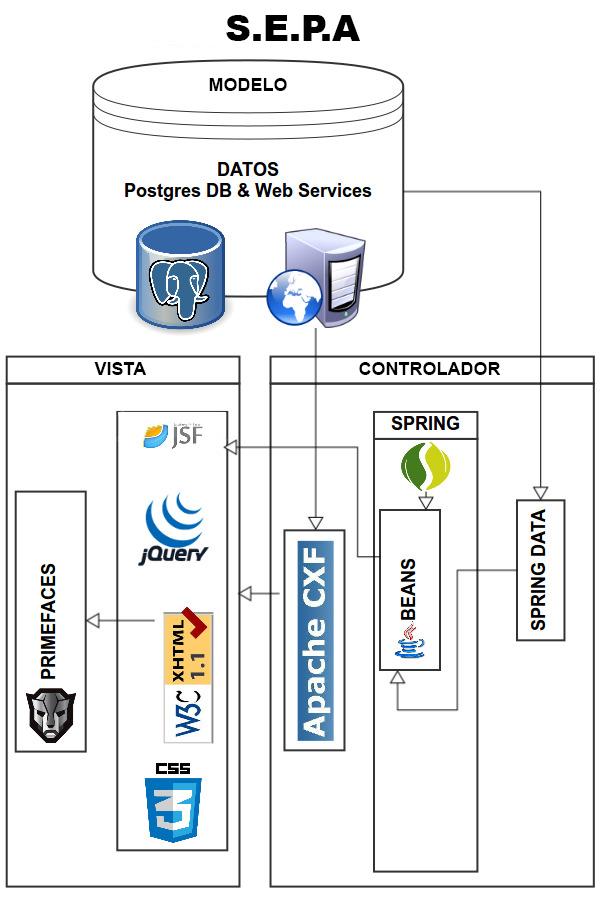
\includegraphics[scale=0.6,angle=0]{images/diagrama.jpg}
\caption{Diagrama general del sistema}
\label{Diagrama general del sistema}
\end{center}
\end{figure}
\chapter{Evaluación de Costos}
\section{Puntos de Función}
Para evaluar los costos monetarios de este proyecto se utilizara el calculo de Puntos de Función para llegar a un valor justificado. Mediante una función matemática que utiliza varios parámetros, divididos en 2 ramas.

\section{Conteo de puntos}

\begin{enumerate}
	\item Ficheros Internos Lógicos (FIL): La información de los datos internos, contenida en bases de datos y ficheros de configuración se tomarán como medida la cantidad de tablas contenidas en el modelo.
	\item Ficheros Externos de Interfaz (FEI): El proyecto utiliza datos externos que son administrados por la aplicación DirDoc. Por ejemplo hay un aproximado de 32 servicios adjuntos al modelo, contenidos en 11 servicios, mas, un aproximado de 24 sub-tareas externas en el integrador contenidas en 6 tareas grandes.
	\item Entrada Externa (EE): El sistema consume servicios web provenientes de otros sistemas.
	\item Salida Externa (SE): El sistema muestra la totalidad de los datos internos en su parte visual. En este caso particular todas las tablas del modelo tienen un apartado visual en la vista.
	\item Consulta Externa (CE): El sistema tiene mantenedores de todos sus datos en base de datos, para poder ser modificables por los usuarios.
\end{enumerate}

\textbf{Tabla de valores ponderados}\\
\begin{tabular}{| l | l | l | l |}
\hline
\textbf{Característica} & \textbf{Ponderación} & \textbf{Valor} & \textbf{Determinante ponderado} \\
\hline
FIL & 49 & medio & 8\\
\hline
FEI & 43 & medio & 3\\
\hline
EE & 16  & alto  & 6\\
\hline
SE & 43  & alto  & 8\\
\hline
CE & 43  & alto  & 8\\
\hline
\end{tabular}
\\\\\\
Los parámetros anteriores deben ser convertidos en distintas tablas.\\
\textbf{Complejidad de los Ficheros}\\
\begin{tabular}{| l | l | l | l |}
\hline
\textbf{RET/DET} & \textbf{1-19} & \textbf{20-50} & \textbf{51+} \\
\hline
1 & Bajo & Bajo & Medio\\
\hline
2-5 & Bajo & Medio & Alto\\
\hline
6+ & Medio & Alto & Alto\\
\hline
\end{tabular}
\\\\\\
\textbf{Complejidad de las Entradas}\\
\begin{tabular}{| l | l | l | l |}
\hline
\textbf{FICH/DET} & \textbf{1-4} & \textbf{5-15} & \textbf{16+} \\
\hline
0-1 & Bajo & Bajo & Medio\\
\hline
2 & Bajo & Medio & Alto\\
\hline
3+ & Medio & Alto & Alto\\
\hline
\end{tabular}
\\\\\\
\textbf{Complejidad de las Salidas}\\
\begin{tabular}{| l | l | l | l |}
\hline
\textbf{FICH/DET} & \textbf{1-5} & \textbf{6-19} & \textbf{20+} \\
\hline
0-1 & Bajo & Bajo & Medio\\
\hline
2-3 & Bajo & Medio & Alto\\
\hline
4+ & Medio & Alto & Alto\\
\hline
\end{tabular}
\\\\\\
\textbf{Tabla de valores calculados}\\
\begin{tabular}{| l | l | l | l | l |}
\hline
\textbf{TIPO} & \textbf{Bajo} & \textbf{Medio} & \textbf{Alto} & \textbf{Total} \\
\hline
EE & x3  & \textbf{8x4}  & x6 & 32\\
\hline
SE & x4  & \textbf{3x5}  & x7 & 15\\
\hline
CE & x3  & x4  & \textbf{6x10} & 60\\
\hline
FIL & x7 & x10 & \textbf{8x25} & 200\\
\hline
FEI & x5 & x7 & \textbf{8x15} & 120\\
\hline
TOTAL &  &  & & 427\\
\hline
\end{tabular}
\\\\\\
El total obtenido debe ser reparado con una serie de factores que se incluyen a continuación.

\section{Características generales del sistema}

En esta sección se evalúa con un número de 0 a 5 las distintas características que este sistema puede o no tener, y finalmente se ponderan para generar un valor que nos permite hacer el ajuste para el conteo de puntos anterior.

\begin{enumerate}
	\item Comunicación de Datos: [4 puntos] Varios teleprocesos pero con el mismo protocolo de comunicaciones.
	\item Proceso Distribuido: [4 puntos] Proceso de datos distribuidos y transferencia de datos en línea en ambas direcciones. Por ejemplo una red de cajeros automáticos en donde estos procesan parte de la transacción.
	\item Objetivos de Rendimiento: [4 puntos] Se utilizan herramientas de análisis de rendimiento durante el diseño, desarrollo e instalación, con el objetivo de alcanzar el rendimiento demandado por el usuario.
	\item Configuración de Explotación Usada intensamente por Otros Sistemas: [1 punto] Existen restricciones, pero son las usuales de cualquier equipo departamental. No es necesario hacer consideraciones especiales.
	\item Tasa de Transacciones: [2 puntos] Se prevén peaks de operaciones semanales.
	\item Entrada de datos EN-LÍNEA: [5 puntos] La entrada de datos interactivas superan el 30 por ciento de las transacciones.
	\item Eficiencia con el Usuario Final: [3 puntos] Seis o más factores, pero sin especiales requerimientos de eficiencia.
	\item Actualizaciones EN-LÍNEA: [4 puntos] Protección ante pérdidas y el sistema se ha de diseñar e implementar con estas consideraciones.
	\item Lógica de Proceso Interno Compleja: [5 puntos] La aplicación llevará incorporados sistemas de seguridad y control.
	\item Reusabilidad del Código: [5 puntos] La aplicación ha sido específicamente empaquetada y/o documentada para ser fácil de reutilizar.
	\item Contempla la Conversión y Facilidad de Instalación: [0 puntos] No reemplazamos un sistema existente o no se requiere conversión. Tampoco se enuncia nada sobre la instalación.
	\item Facilidad de Operación: [5 puntos] Sistema automático sin intervención humana.
	\item Instalaciones Múltiples: [3 puntos] La aplicación correrá en múltiples entornos de Hw o Sw y se tiene en cuenta desde la fase de diseño.
	\item Facilidad de Cambios: [3 puntos] El cambio de la configuración se hace interactivamente y tiene efecto inmediato.
\end{enumerate}

\textbf{Cálculo de los puntos de función ajustados}\\
\begin{tabular}{| l | l | l |}
\hline
\textbf{No.} & \textbf{Factor de Complejidad} & \textbf{Valor}\\
\hline
1 &  Comunicación de Datos & 4 \\
\hline
2 &  Proceso Distribuido &4  \\
\hline
3 & Objetivos de Rendimiento  &4  \\
\hline
4 & Configuración Explotación Compartida  & 1 \\
\hline
5 & Tasa de Transacciones  & 2 \\
\hline
6 &  Entrada de Datos EN-LÍNEA &  5\\
\hline
7 & Eficiencia con el Usuario Final  &  3\\
\hline
8 & Actualizaciones En-LÍNEA  & 4 \\
\hline
9 & Lógica del Proceso Interno Compleja  &  5\\
\hline
10 & Reusabilidad del Código  &  5\\
\hline
11&  Contempla la Conversión e Instalación &  0\\
\hline
12& Facilidad de Operación  &  5\\
\hline
13& Instalaciones Múltiples  &  3\\
\hline
14& Facilidad de Cambios  & 3 \\
\hline
\multicolumn{2}{|c|}{Factor de Complejidad Total (FCT)} & 48\\
\hline
\end{tabular}
\\\\\\

\section{Puntos de función ajustados}
La siguiente fórmula describe la cantidad ajustada de puntos de función y éstos a su vez son multiplicados por el valor en horas dando lo que cuesta en tiempo y dinero, cada uno de los puntos obteniéndose finalmente el valor ponderado del proyecto en sí.

\begin{math}
PFA=PFSA * ( 0.65 + ( 0.01 * FCT ) = 427 * ( 0.65 + ( 0.01 * 48 ) = 452.51
\end{math}

Después se multiplican los Puntos de Función por un factor de 4 horas hombre por cada punto de función.

\begin{math}
452.51 PF * 4 (HH / PF) = 452.51 * (4) = 1810.04 HH
\end{math}

Finalmente se multiplican las horas hombre por el factor 0.4 UF / HH.

\begin{math}
1810.04 HH * 0.4(UF / HH) = 724.016 UF = 17.492.226.6 \$
\end{math}

El proyecto tiene un costo mínimo de 17.500.000 pesos.

\chapter{Conclusiones}

\section{Garantías de calidad}

La calidad de este sistema se ve potenciada por varios aspectos, los cuales se explicaran a continuación:

\begin{enumerate}
        \item Uso de una base de datos PostgreSQL: Un sistema gestor de bases de datos, de código abierto, echo para ser una potente forma de mantener grandes cantidades de datos. Siendo un proyecto realizado de manera altruista por muchos desarrolladores a nivel mundial, es muy estable, seguro y es el entorno necesario para que el sistema S.E.P.A. trabaje sin necesidad de pensar en licencias u otros tipos de registros de datos. Contiene una infinidad de tipos de datos que fortalece la forma de como uno ingresa parámetros.
        \item Uso de Mybatis: Herramienta de ayuda para sentencias SQL que permite el uso de cualquier base de datos, con gran escalabilidad y adaptabilidad, permitiendo escribir las consultas que uno desee ejecutar y mapearlas directamente en los objetos que uno desee. Tiene un nivel de complejidad medio, lo que hace que sea un poco difícil aprender, pero una ves se comprende, la incorporación de nuevos elementos de data es ordenada y escalable.
        \item Uso de WebServices: Una tecnología que utiliza un conjunto de protocolos y estándares que sirven para intercambiar datos entre aplicaciones. Distintas aplicaciones de software desarrolladas en lenguajes de programación diferentes, y ejecutadas sobre cualquier plataforma, pueden utilizar los servicios web para intercambiar datos en redes de ordenadores como Internet.
        \item Uso de Primefaces: Una librería de componentes para JavaServer Faces (JSF) de código abierto que cuenta con un conjunto de componentes enriquecidos que facilitan la creación de las aplicaciones web. Soporte de ajax con despliegue parcial, lo que permite controlar qué componentes de la página actual se actualizarán y cuáles no.
        \item Uso de Metodología de Trabajo: El uso de PSP fortalece el desempeño del proyecto, mostrando los errores que el proceso de desarrollo pueda presentar, desde esta perspectiva es necesario destacar que cuando se van anotando los errores éstos tienden a disminuir con el tiempo por lo que en las etapas finales es muy difícil encontrar errores en el desarrollo.
        \item Uso de Patrón de diseño: El patrón MVC ha hecho de este proyecto un ente robusto y consistente que puede ser mejorable incluso con poco conocimiento, ya que posee una base sólida que sustenta su funcionamiento, por lo cual los cambios que se puedan necesitar en el futuro harán uso de las herramientas que se fabricaron el desarrollo mismo.
        \item Uso de Java y Frameworks: Esto nos permite una autonomía en varios aspectos, ya que nosotros como impulsores de proyectos tenemos siempre que velar por que todo el desarrollo sea altamente eficiente, y una manera muy clara de obtener eso es mediante el uso de herramientas que ya han sido muy probadas y se encuentran en uso de muchos otros proyectos. Dado que en otros sistemas esto ha funcionado muy bien es de esperar que en el nuestro también funcione de igual modo.
        \item Pruebas de rendimiento: Las pruebas sobrecargan el sistema de tal manera que nos permiten decir a ciencia cierta si el software es capaz de resistir lo que los datos nos entregan, y estas nos demuestran que el trabajo realizado cumple con ciertas características que cumple un proyecto web de gran valor.
\end{enumerate}

Finalmente con de estos puntos se puede tener una clara idea de la calidad del producto que se entrega y de cómo éste puede ir mejorando todavía, e inclusive puede cambiar y adecuase a otras necesidades.

\section{Conclusión}
El trabajo correspondiente al Sistema Mantenedor e Integrador en S.E.P.A. ha mostrado como recuperar datos que pueden ser difíciles de manejar. Los datos para este trabajo no estaban del todo bien organizados, esto quiere decir que cuando uno observa los datos, es posible encontrar insuficiencias de campos en los objetos mostrados en las tablas de los mantenedores, para lo cual los Mantenedores están preparados para ingresar datos en los sectores que lo requieran.

También es posible identificar errores estructurales de información. Por ejemplo, en el sistema Integrador entraban datos que contenían errores repetidos en todas las filas de ciertas tablas. Este sistema está preparado para resistir ese tipo de datos y cargar una data estándar que más adelante será reparada por el sistema Mantenedor.

Un proyecto de estas características es una importante oportunidad de mejoras, tales como: mantenibilidad de la data, aunque esta contenga errores, ya que es posible editar aspectos mínimos dentro de todas las tablas, conectividad con servicios web, manejado por parámetros SOAP, dejando la complejidad de las comunicaciones a frameworks que se encargan de trabajar con estas interacciones.

Gracias a este trabajo se puede hablar de indicadores estadísticos, los cuales nos proporcionan información que regulan el funcionamiento de cualquier organización. Para este caso en particular, el desarrollo de indicadores, nos permite sostener una organización a nivel de estudiantes, integrando consultas estadísticas a problemas particulares en estudiantes y profesores. Principalmente el objetivo de S.E.P.A. era ser mostrado.

La ventaja de que este sistema se comunique con otros mediante el uso de WebServices es que a lo largo de la vida útil de este proyecto se pueden agregar otros proyectos que pueden nutriste de la información que S.E.P.A. produce, de tal manera hace que cada ves sea mas intenso su uso.
\section{Trabajo Futuro}
Para ampliar las posibilidades de un trabajo que descansa sobre el valor de potenciar las capacidades administrativas de una institución académica, es necesario hacer estudios que posibiliten un mayor alcance de datos, tal como lo hace S.E.P.A., por tal razón es de vital importancia promover nuevas mejoras que hagan de este sistema una herramienta completa en el desarrollo de las capacidades generales de una organización, como lo es la Universidad Tecnológica Metropolitana.

Se puede considerar el integrar un motor de minería de datos que revele información que hasta ahora no se ha obtenido dentro de los marcos de este proyecto, por ejemplo, una herramienta que obtenga formulaciones o métodos de aproximación para datos del futuro. Tal cosa produciría un impacto en S.E.P.A. ya que con esta perspectiva se aumentan los beneficios de los indicadores que uno puede obtener, validando estos o creando aproximaciones que ayudan a esclarecer las razones de los valores que actualmente entrega el sistema.

También se piensa en una Inteligencia de Negocio que junto con la idea anterior sea capaz de producir nuevos indicadores enfocados a la mejora o a la conducción, con intervención humana, de los valores generalizados en las tablas que maneja S.E.P.A., en otras palabras, que se sepa información que nos permitiera guiar a la Universidad en torno a los objetivos de su Visión, haciendo un impacto en el corto plazo.

Estas dos ideas anteriores convergen finalmente en que el sistema en un futuro podría tener una Inteligencia Artificial que sea manejable por los usuarios de S.E.P.A. permitiendo manejar las respuestas de los usuarios en pos de darle las mejores oportunidades a todos por igual. Mediando en todos los asuntos de manera logia, estadística y totalmente regulada. Podríamos decir que en un futuro, S.E.P.A. seria un sistema automático y autónomo.

Finalizando, se puede afirmar que un trabajo como éste es perfectamente capaz de entregar datos y argumentos sólidos en pos de generar estudios científicos relacionados con indicadores de calidad en educación, puesto que con el sistema S.E.P.A. en las condiciones actuales mejoradas, se tienen todas las herramientas preparadas para tales propósitos. 
\bibliographystyle{plain}
\bibliography{bibliografia.bib}
\end{document}